\apendice{Especificación de diseño}

\section{Introducción}
Una vez tenemos bien definidos los requisitos funcionales y los casos de uso, tenemos que realizar las diferentes tareas de diseño necesarias para poder transformar esos requisitos que ha definido el cliente, en software tangible y bien elaborado.

En este apartado voy a comentar los distintos diseños que he realizado para el desarrollo dele proyecto, estos tipos de diseño son:
\begin{itemize}
	\item \textbf{Diseño de datos:} en el cual voy a explicar los diseños y decisiones referentes a las estructuras de datos y a los propios datos.
	\item \textbf{Diseño procedimental:} explicación detallada de como se relacionan los apartados en la ejecución, con diagramas de secuencia.
	\item \textbf{Diseño arquitectónico:} explicación de las relaciones entre las distintas partes del sistema.
	\item \textbf{Diseño de interfaces:} donde se podrá ver como se ha diseñado las interfaces y sus versiones iniciales.
	\item \textbf{Diseño de código de errores:} donde explicaré la estandarización que se ha realizado para controlar los errores de la conexión entre la aplicación y el servidor.
\end{itemize}
\section{Diseño de datos}
En este subapartado voy a comentar los distintos aspectos de diseños relacionado con los datos, es decir, como se organizan y de que están compuestos.

Cabe destacar que ambas aplicaciones \textit{Android}, trabajan sobre una carpeta raíz base llamada \textit{Apace}, que si no existe al iniciar la aplicación se crea automaticamente.

\subsection{Aplicación de Recogida de Datos}
En esta aplicación lo que hacemos es generar datos para poder comprimirlos y después enviarlos por correo para su posterior investigación. Estos datos están compuestos de un audio con un sonido de una persona con parálisis cerebral gravemente afectada, unas opciones adiciones y el resultado que la persona que ha grabado cree que es.

Para poder generar todos estos datos ha de existir una forma de poder, dentro de nuestro dispositivo \textit{Android}, crear carpetas donde poder guardar nuestros datos para posteriormente comprimirlos y enviarlos. En esta aplicación, cada vez que seleccionamos un paciente y entramos en la pantalla de grabar un audio se crea una carpeta con el nombre del paciente y la fecha, con hora y segundos. Por cada uno de los ficheros que creamos en una misma ejecución, se almacenan en esta carpeta con el mismo nombre más un valor identificativo. Cabe destacar que para los ficheros en donde se almacenan las opciones adiciones y el resultado (emociones o respuesta) están almacenados en ficheros csv.

Una vez tenemos todos los datos creados en la carpeta, al enviar se genera un comprimido con el mismo nombre de la carpeta donde están los datos y se envía.

Un ejemplo de la estructura de datos comentada sería:

\dirtree{%
	.1 Apace.
	.2 JMiguel\_10-35-36\_19-06-2019.
	.3 JMiguel\_10-35-36\_19-06-2019.mp4.
	.3 JMiguel\_10-35-36\_19-06-2019\_Estado.csv.
	.3 JMiguel\_10-35-36\_19-06-2019\_Opciones.csv.
	.2 JMiguel\_10-35-36\_19-06-2019.zip.
}

Donde podemos ver que de la carpeta generada cuelgan los ficheros del audio, las opciones adicionales y las emociones o respuestas relacionadas. Y que después se ha generado el comprimido a partir de esta carpeta con el mismo nombre, con formato \textit{zip}.
\subsection{Aplicación para la Interpretación}
Esta segunda aplicación es bastante más compleja, en cuanto a la lógica que hay detrás, como al conjunto de datos que maneja.

En primer lugar voy a comentar la estructura de ficheros con la que trabaja la aplicación. En esta aplicación, si no existe algún fichero y/o carpeta en la creación se crea automaticamente gracias al método \textit{inicio()} que se ejecuta nada más crear el primer \textit{Activity}, el \textit{MainActivity}. La estructura de ficheros que da soporte a la lógica de la aplicación es la siguiente:

\dirtree{%
	.1 Apace.
	.2 JMiguel\_10-35-36\_19-06-2019.mp4.
	.2 config.
	.3 paciente.csv.
}

En esta estructura nos encontramos con una carpeta \textit{config}, que es donde se almacenan los fichero de configuración, como lo es el fichero \textit{paciente.csv} que nos permite almacenar el último paciente seleccionado en la última ejecución, el cual será cargado en el siguiente inicio de la aplicación, para así tener un paciente por defecto.

Como se puede observar, del directorio raíz también cuelga un fichero \textit{mp4}, este es un ejemplo de donde se almacenan los audios antes de ser enviados al servidor para interpretar. No es hasta que hemos obtenido el resultado de la interpretación cuando este fichero se elimina, para así ocupar el menor almacenamiento posible.

Pero la estructura de datos no es la única parte relevante en el diseño de los datos de una aplicación, sino que también lo son las clases con las que trabajamos, como se puede ver en la figura~\ref{fig:clases}. Como se puede ver en el diagrama, trabajamos con un conjunto grande de clases, cada una con los datos necesarios para realizar sus funcionalidad.

\begin{figure}[H]
	\centering
	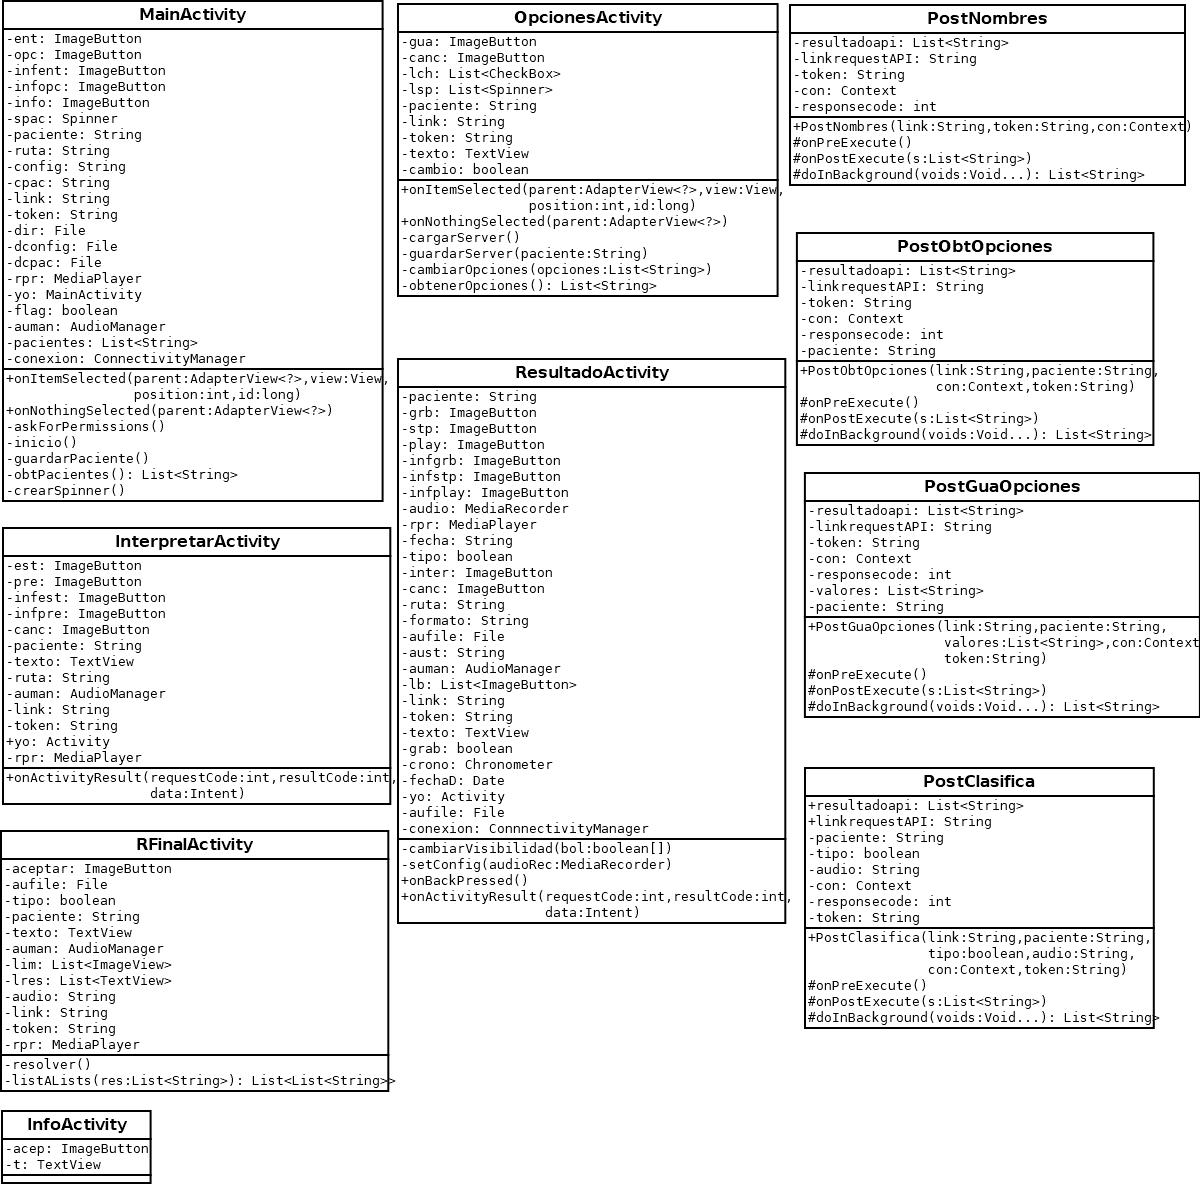
\includegraphics[width=\textwidth]{clases}
	\caption{Diagrama de clases.}
	\label{fig:clases}
\end{figure}

Aun con las estructuras de datos de la aplicación y el diagrama de clases no hemos terminado con el diseño de los datos, ya que una parte muy importante de esta es ver la relación que existe entre las diferentes clases, estas relaciones las podemos ver en el diagrama de clases de alto nivel en la figura~\ref{fig:clasesal}.

\begin{figure}[H]
	\centering
	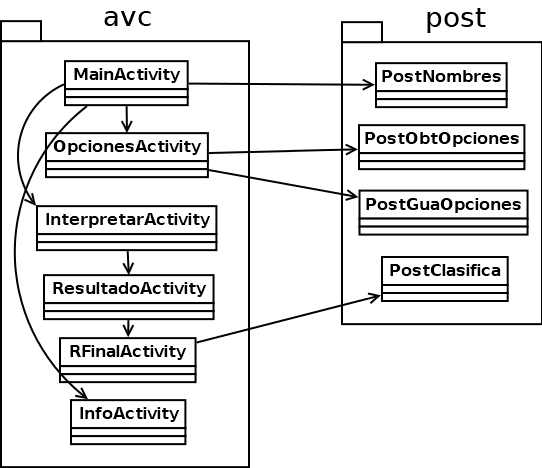
\includegraphics[width=\textwidth]{clasesal}
	\caption{Diagrama de Clases de Alto Nivel.}
	\label{fig:clasesal}
\end{figure}

En el diagrama se representan las llamadas entre las diferentes clases, habiendo en estas llamadas distintos parámetros como puede ser la \textit{url} del servidor, el \textit{token} de seguridad o el paciente seleccionado.

\subsection{Servidor} \label{server}
Dentro del servidor, como ya se ha comentado en la memoria, se ha puesto un especial interés en el diseño y en la creación de la estructura de datos que nos permita controlar los datos que maneja el servidor. Esta estructura es la siguiente:
\dirtree{%
	.1 root.
	.2 Modelos.
	.2 Opciones.
	.2 Temp.
	.2 pacientes.csv.
	.2 apiserver.py.
	.2 clip.py.
}

En la carpeta \textit{Modelos}, es donde nos encontramos con los modelos entrenados de los pacientes, tanto los modelos para interpretar estados como los modelos para interpretar respuesta. En la carpeta \textit{Opciones} se encuentran los distintos archivos con los valores actuales de las opciones adicionales de los pacientes. Por último, en la carpeta \textit{Temp} es donde se almacenan los audios subidos desde la aplicación móvil, que una vez el servidor realiza la respuesta al cliente este audio se elimina.
\newpage
\section{Diseño procedimental}
\subsection{Aplicación para la recogida de datos}
En esta aplicación solo hay un procedimiento de ejecución, ya que es lo que se quería, una aplicación con una ejecución lineal, que resultase fácil de utilizar para los usuarios, como así nos comentaron en las distintas presentaciones de esta aplicación. El procedimiento de esta ejecución se puede ver en el diagrama de secuencia simplificado en la figura~\ref{fig:dsgd} y en el diagrama de secuencia normal en la figura~\ref{fig:dsgd2}.

\begin{figure}[H]
	\centering
	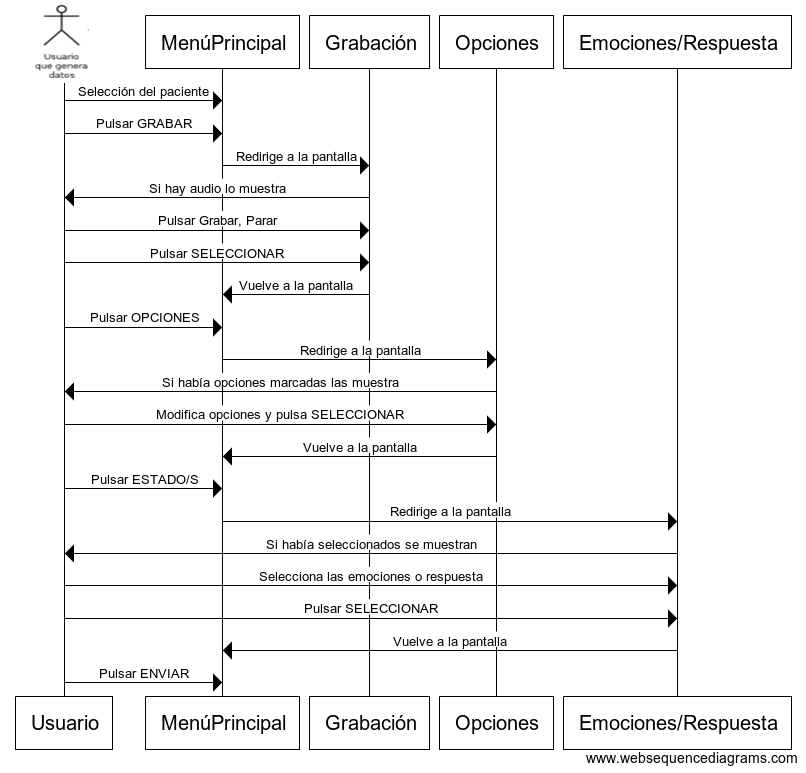
\includegraphics[width=\textwidth]{dsgd}
	\caption{Diagrama de Secuencia simplificado aplicación generación de datos.}
	\label{fig:dsgd}
\end{figure}

\begin{figure}[H]
	\centering
	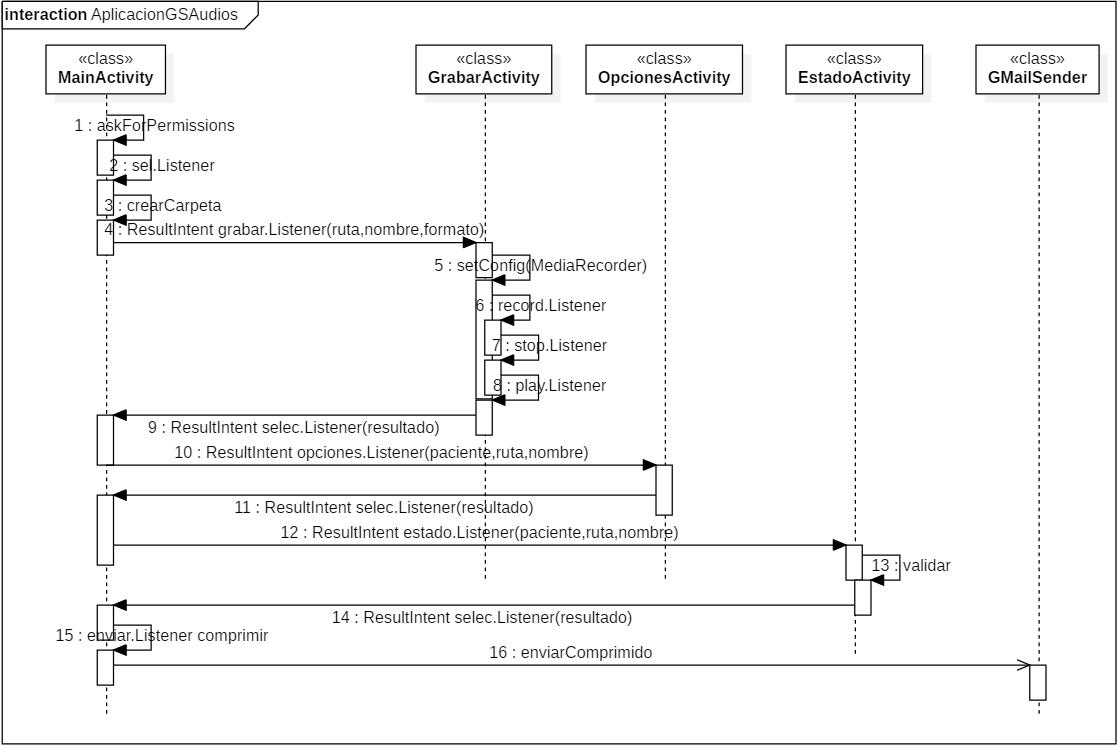
\includegraphics[width=\textwidth]{dsgd2}
	\caption{Diagrama de Secuencia aplicación generación de datos.}
	\label{fig:dsgd2}
\end{figure}

\subsection{Aplicación para la interpretación}
Hay distintas procedimientos que podemos probar en la aplicación de interpretación, estos son unos procedimientos bien definidos que nos permiten realizar las distintas funcionalidades que tiene esta aplicación y el servidor al que está conectado.

Estos procedimientos han sido diseñados siguiendo los diagramas de secuencia simplificados que se pueden ver en las figuras~\ref{fig:ds1},~\ref{fig:ds2},~\ref{fig:ds3} y ~\ref{fig:ds4}. También se ha seguido los diagramas de secuencias que se pueden ver en las figuras~\ref{fig:ds1n},~\ref{fig:ds2n} y~\ref{fig:ds3n}.

\begin{figure}[htp]
	\centering
	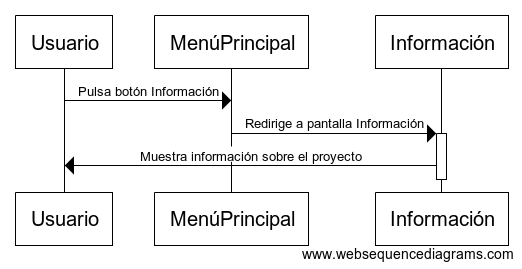
\includegraphics[width=\textwidth]{ds1}
	\caption{Diagrama de Secuencia simplificado de Información.}
	\label{fig:ds1}
\end{figure}

\begin{figure}[htp]
	\centering
	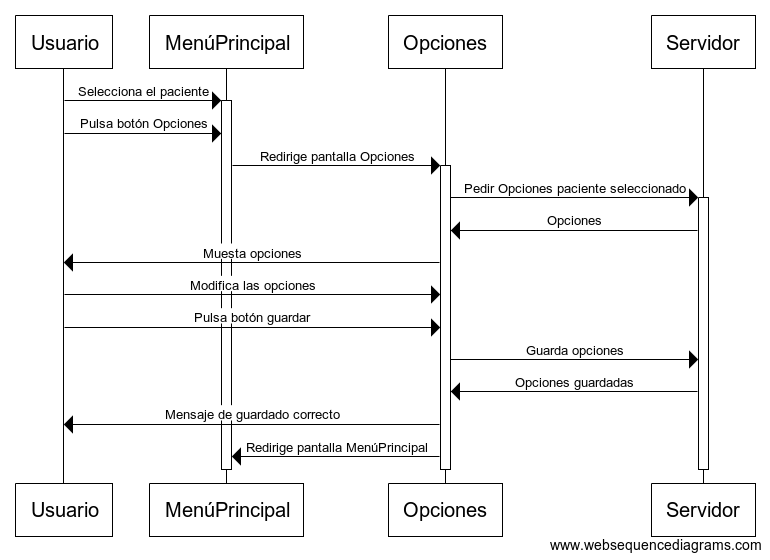
\includegraphics[width=\textwidth]{ds2}
	\caption{Diagrama de Secuencia simplificado del cambio de las opciones.}
	\label{fig:ds2}
\end{figure}

\begin{figure}[htp]
	\centering
	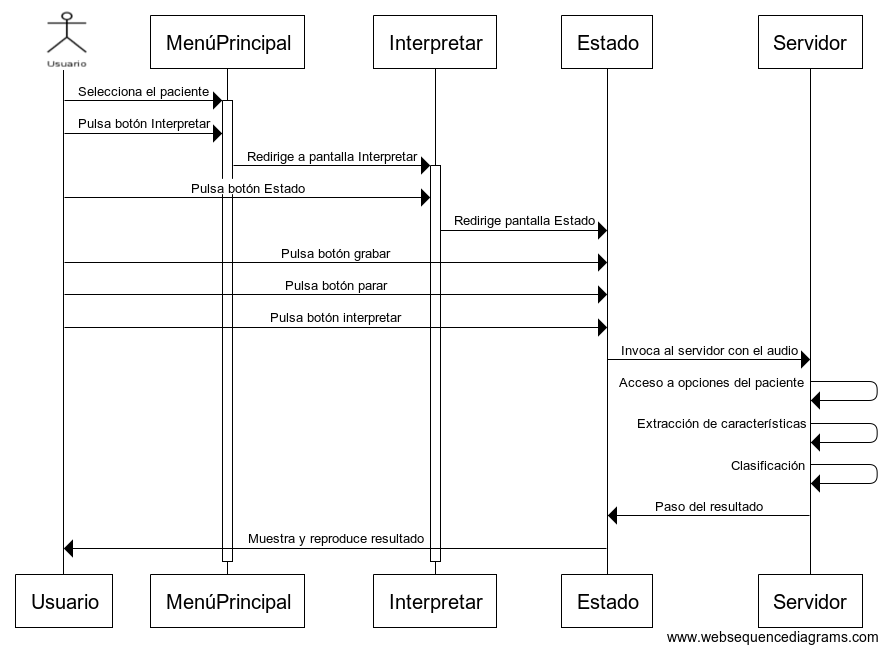
\includegraphics[width=\textwidth]{ds3}
	\caption{Diagrama de Secuencia simplificado de la interpretación de una emoción/estado.}
	\label{fig:ds3}
\end{figure}

\begin{figure}[htp]
	\centering
	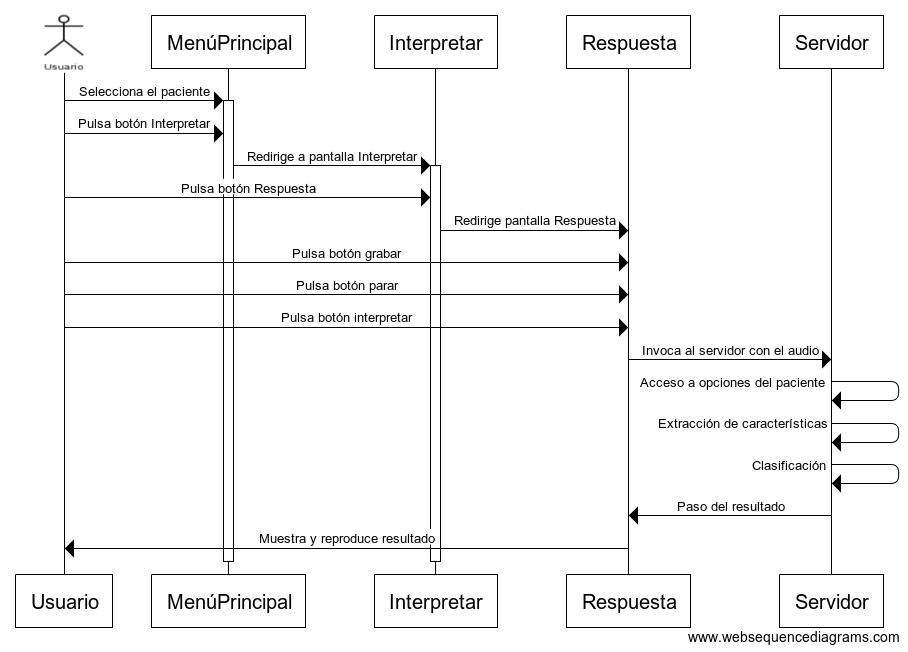
\includegraphics[width=\textwidth]{ds4}
	\caption{Diagrama de Secuencia de la interpretación de una respuesta.}
	\label{fig:ds4}
\end{figure}

\begin{figure}[htp]
	\centering
	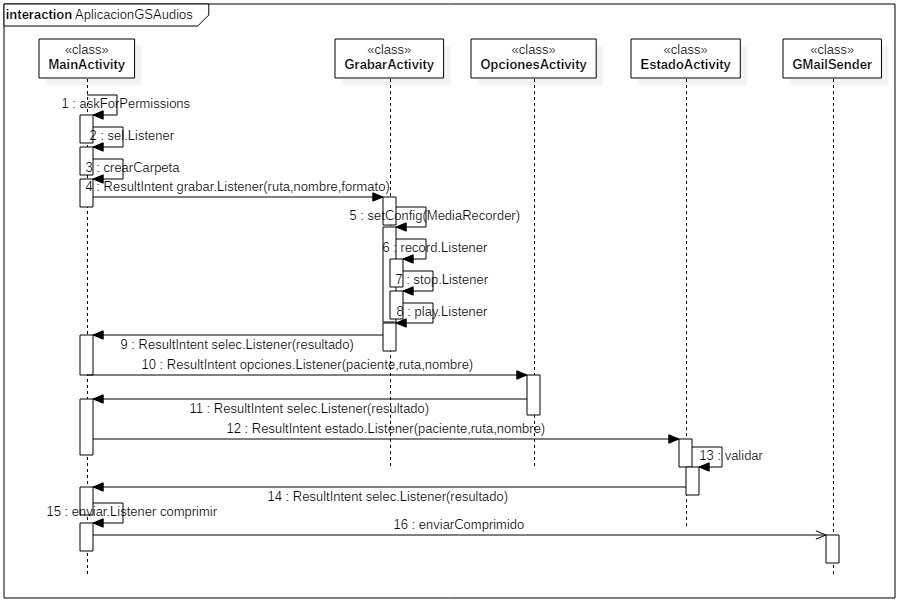
\includegraphics[width=\textwidth]{ds1n}
	\caption{Diagrama de Secuencia de Información.}
	\label{fig:ds1n}
\end{figure}

\begin{figure}[htp]
	\centering
	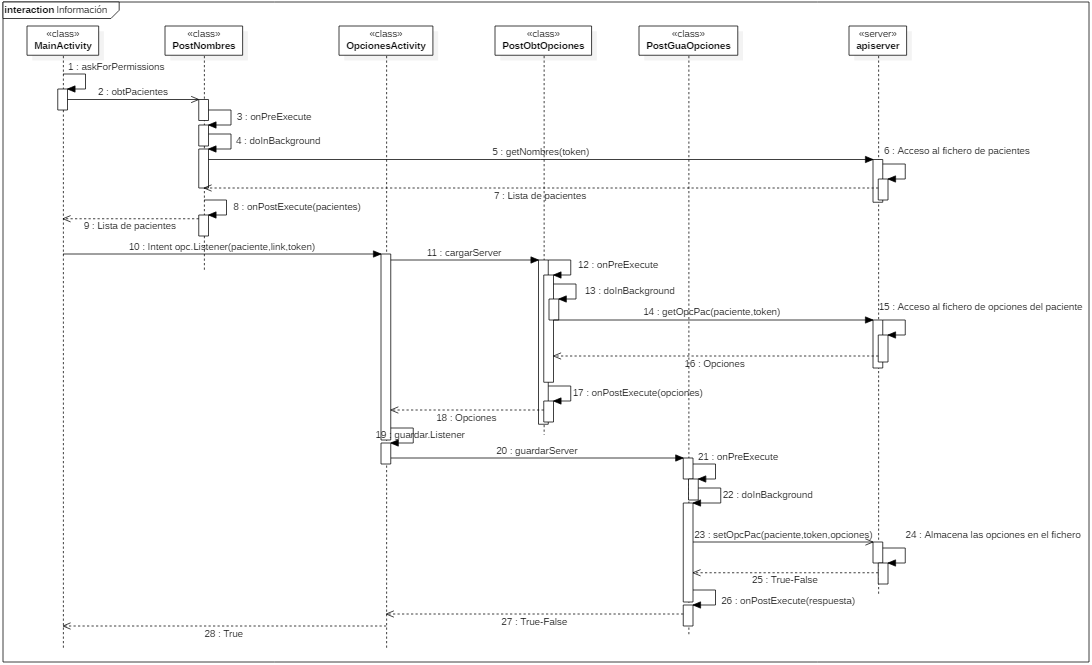
\includegraphics[width=\textwidth]{ds2n}
	\caption{Diagrama de Secuencia del cambio de las opciones.}
	\label{fig:ds2n}
\end{figure}

\begin{figure}[H]
	\centering
	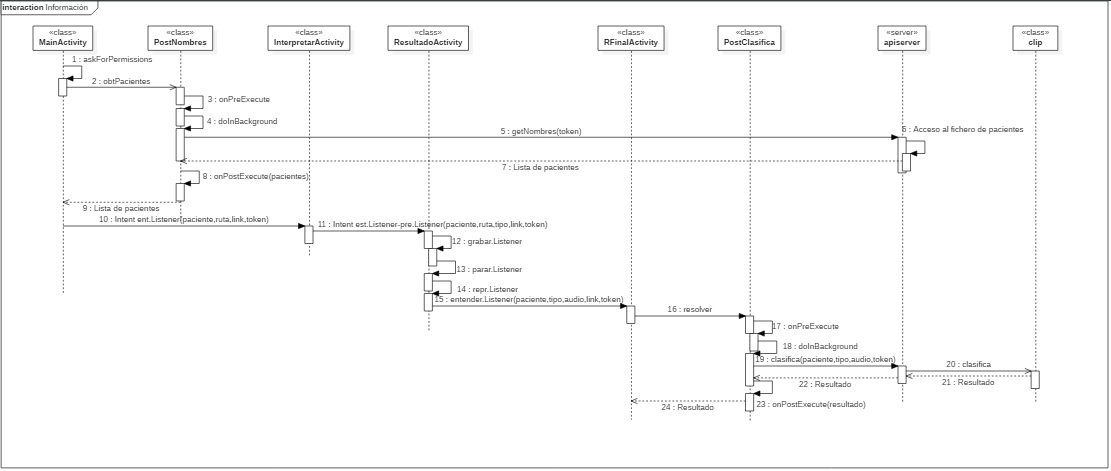
\includegraphics[width=\textwidth]{ds3n}
	\caption{Diagrama de Secuencia de la interpretación.}
	\label{fig:ds3n}
\end{figure}

Como se puede ver, cada diagrama muestra el diseño de una parte de la aplicación, en el primer diagrama, figura~\ref{fig:ds1} podemos ver la secuencia para llegar a la pantalla de información del proyecto. En el segundo diagrama, figura~\ref{fig:ds2}, se puede ver la secuencia de procesos que hay que realizar para poder modificar las opciones de un paciente. Por último, podemos ver en los diagramas de la secuencia de pasos a seguir para poder interpretar una emoción, figura~\ref{fig:ds3}, y una respuesta, figura~\ref{fig:ds4}. 
\section{Diseño arquitectónico}

Como se he comentado a lo largo de la memoria y de los anexos, en el proyecto se han desarrollado distintas aplicaciones y una servidor, que conforman un sistema en el cual una aplicación genera datos que sirven para crear clasificadores con los que poder interpretar en el servidor, sonidos capturados desde la aplicación de interpretación.

La relación entre las distintas partes con conforman el sistema se puede ver en la figura~\ref{fig:dsal}.

\begin{figure}
	\centering
	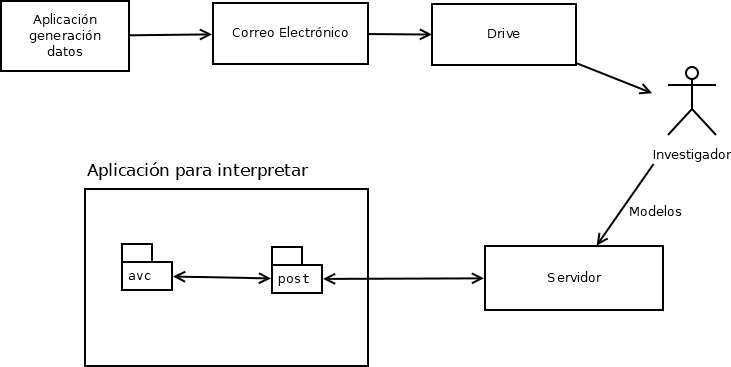
\includegraphics[width=\textwidth]{dsal}
	\caption{Diagrama de Secuencia de Alto Nivel.}
	\label{fig:dsal}
\end{figure}

Como se puede observar, hay dos líneas de ejecución. Una que nos permite generar datos, en la cual partimos de las grabaciones obtenidas de la aplicación de generación de datos, estos datos son enviados por correo y recogidos en drive para que posteriormente el investigador colaborador, Sergio Chico, pueda trabajar y obtener los mejores algoritmos de extracción de características y de clasificación. Por otro lado, tenemos la ejecución orientada a la interpretación, esta comienza con la grabación de los audios en la aplicación para interpretar, en concreto en el paquete \textit{avc}, que luego llama a las clases del paquete \textit{post} para comunicarse con el servidor y obtener el resultado de la interpretación.
\section{Diseño de interfaces}
Otra parte muy importante en el desarrollo de un proyecto es el diseño de las interfaces de los programas y aplicaciones que se desarrollen. Es más importante aun si tienes un cliente que te contrata para realizar el proyecto, ya que la interfaz tiene que estar cuidadosamente diseñada para cumplir con sus requisitos.
\subsection{Aplicación de generación de datos}
El diseño de la interfaz que hice de esta aplicación se puede ver en la figura~\ref{fig:digd}. Y la interfaz final de la aplicación se puede ver en la figura~\ref{fig:digdfinal}.
\begin{figure}
	\centering
	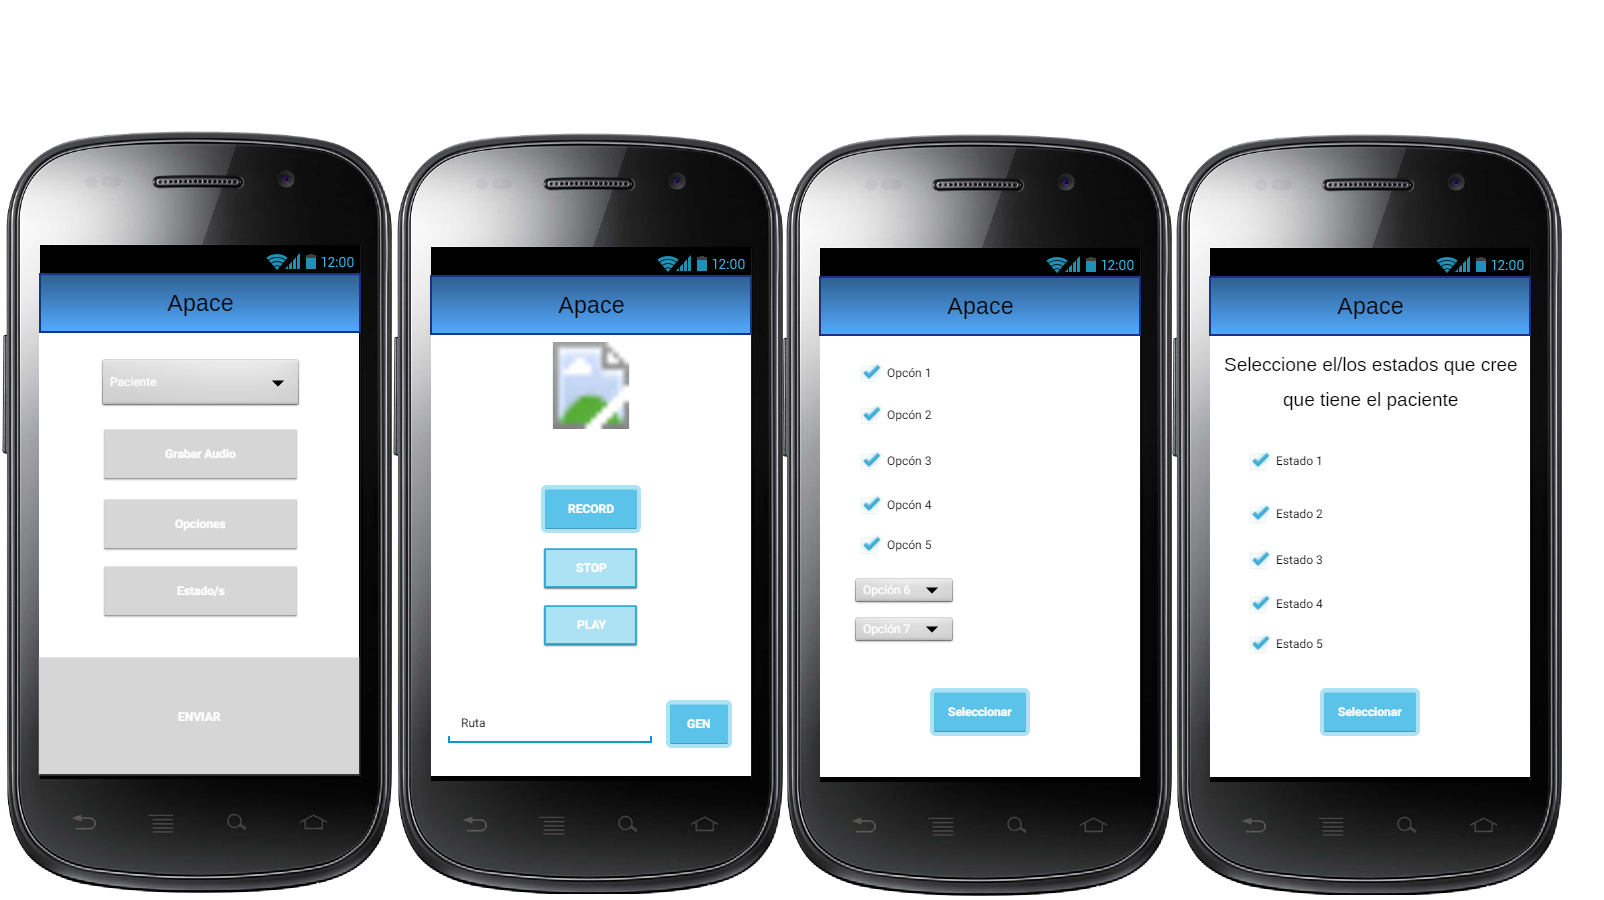
\includegraphics[width=\textwidth]{interfaz}
	\caption{Diseño interfaz aplicación recogida de datos.}
	\label{fig:digd}
\end{figure}

\begin{figure}
	\centering
	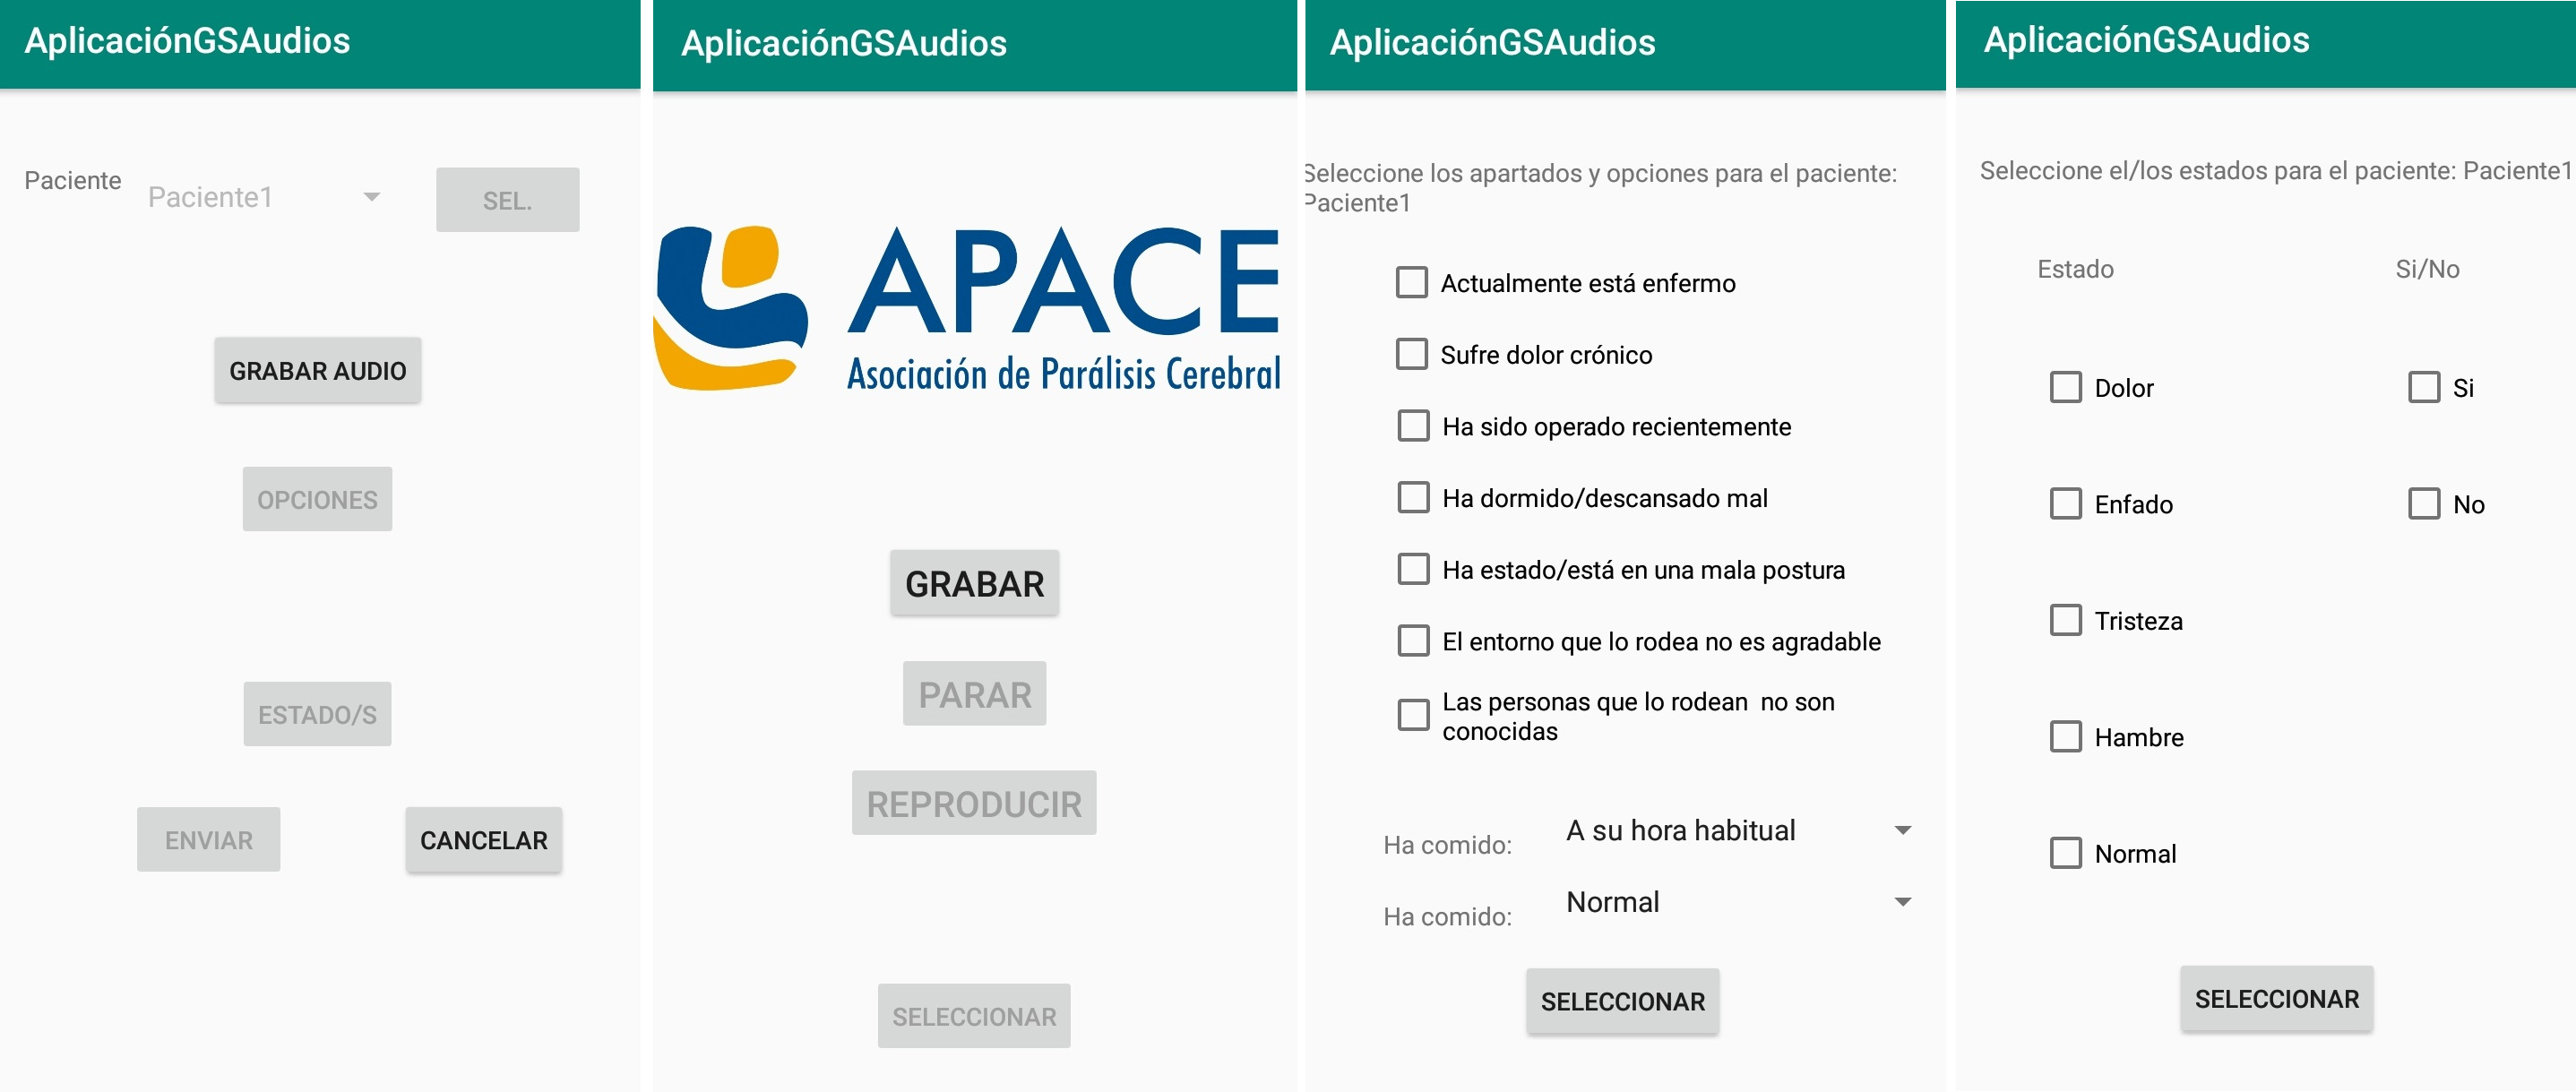
\includegraphics[width=\textwidth]{interfinalrd}
	\caption{Interfaz final de la aplicación recogida de datos.}
	\label{fig:digdfinal}
\end{figure}

\subsection{Aplicación para interpretar}
En esta aplicación se puso mucho empeño en realizar un buen diseño, y junto con el equipo de APACE Burgos diseñamos al rededor de 8 interfaces, de las cuales se eligió la interfaz que se puede ver en la figura~\ref{fig:diinter}.

A la aplicación final llegaron muchos cambios, algunos pedidos por APACE Burgos y otros por meras necesidades que veía al ver la interfaz. Entre los cambios más significativos están el cambio de color de los botones, o la disposición de alguna pantalla. La interfaz final de la aplicación se puede ver en la figura~\ref{fig:intfin}.

\begin{figure}[htp]
	\centering
	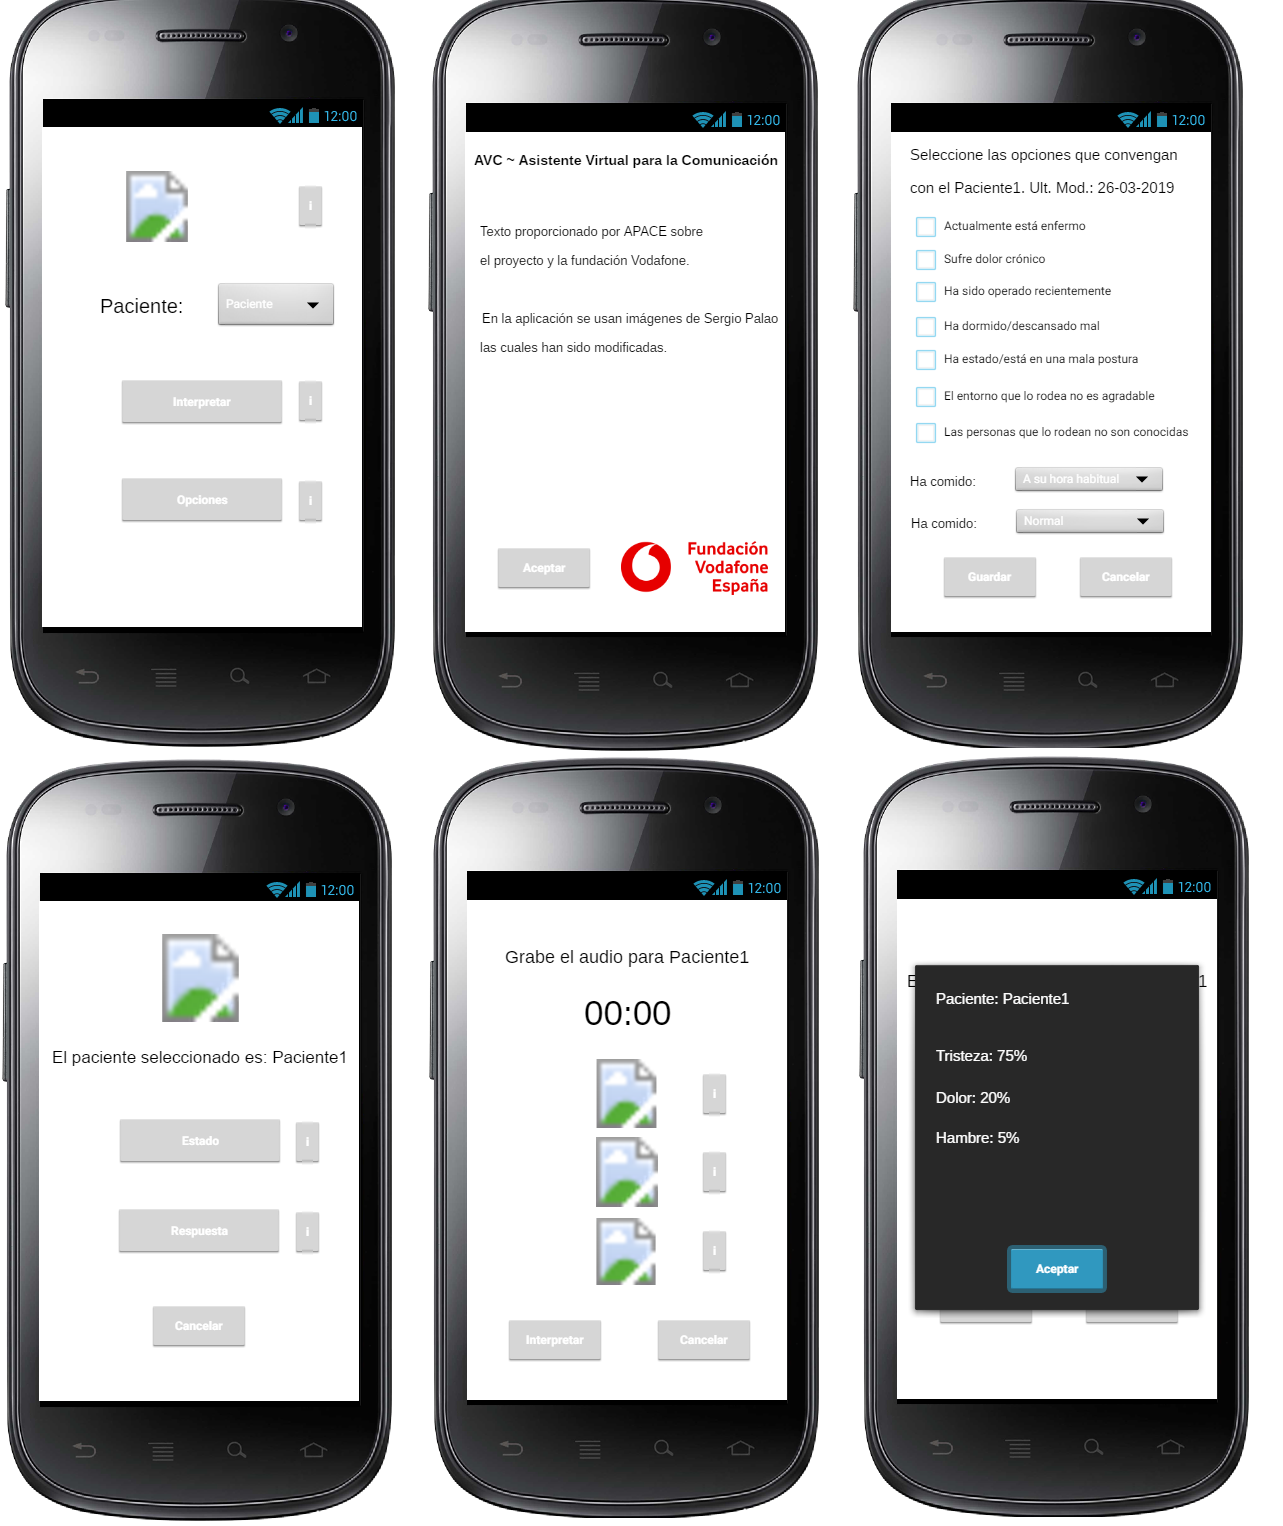
\includegraphics[width=\textwidth]{disintavc}
	\caption{Diseño interfaz aplicación interpretación.}
	\label{fig:diinter}
\end{figure}

\begin{figure}[H]
	\centering
	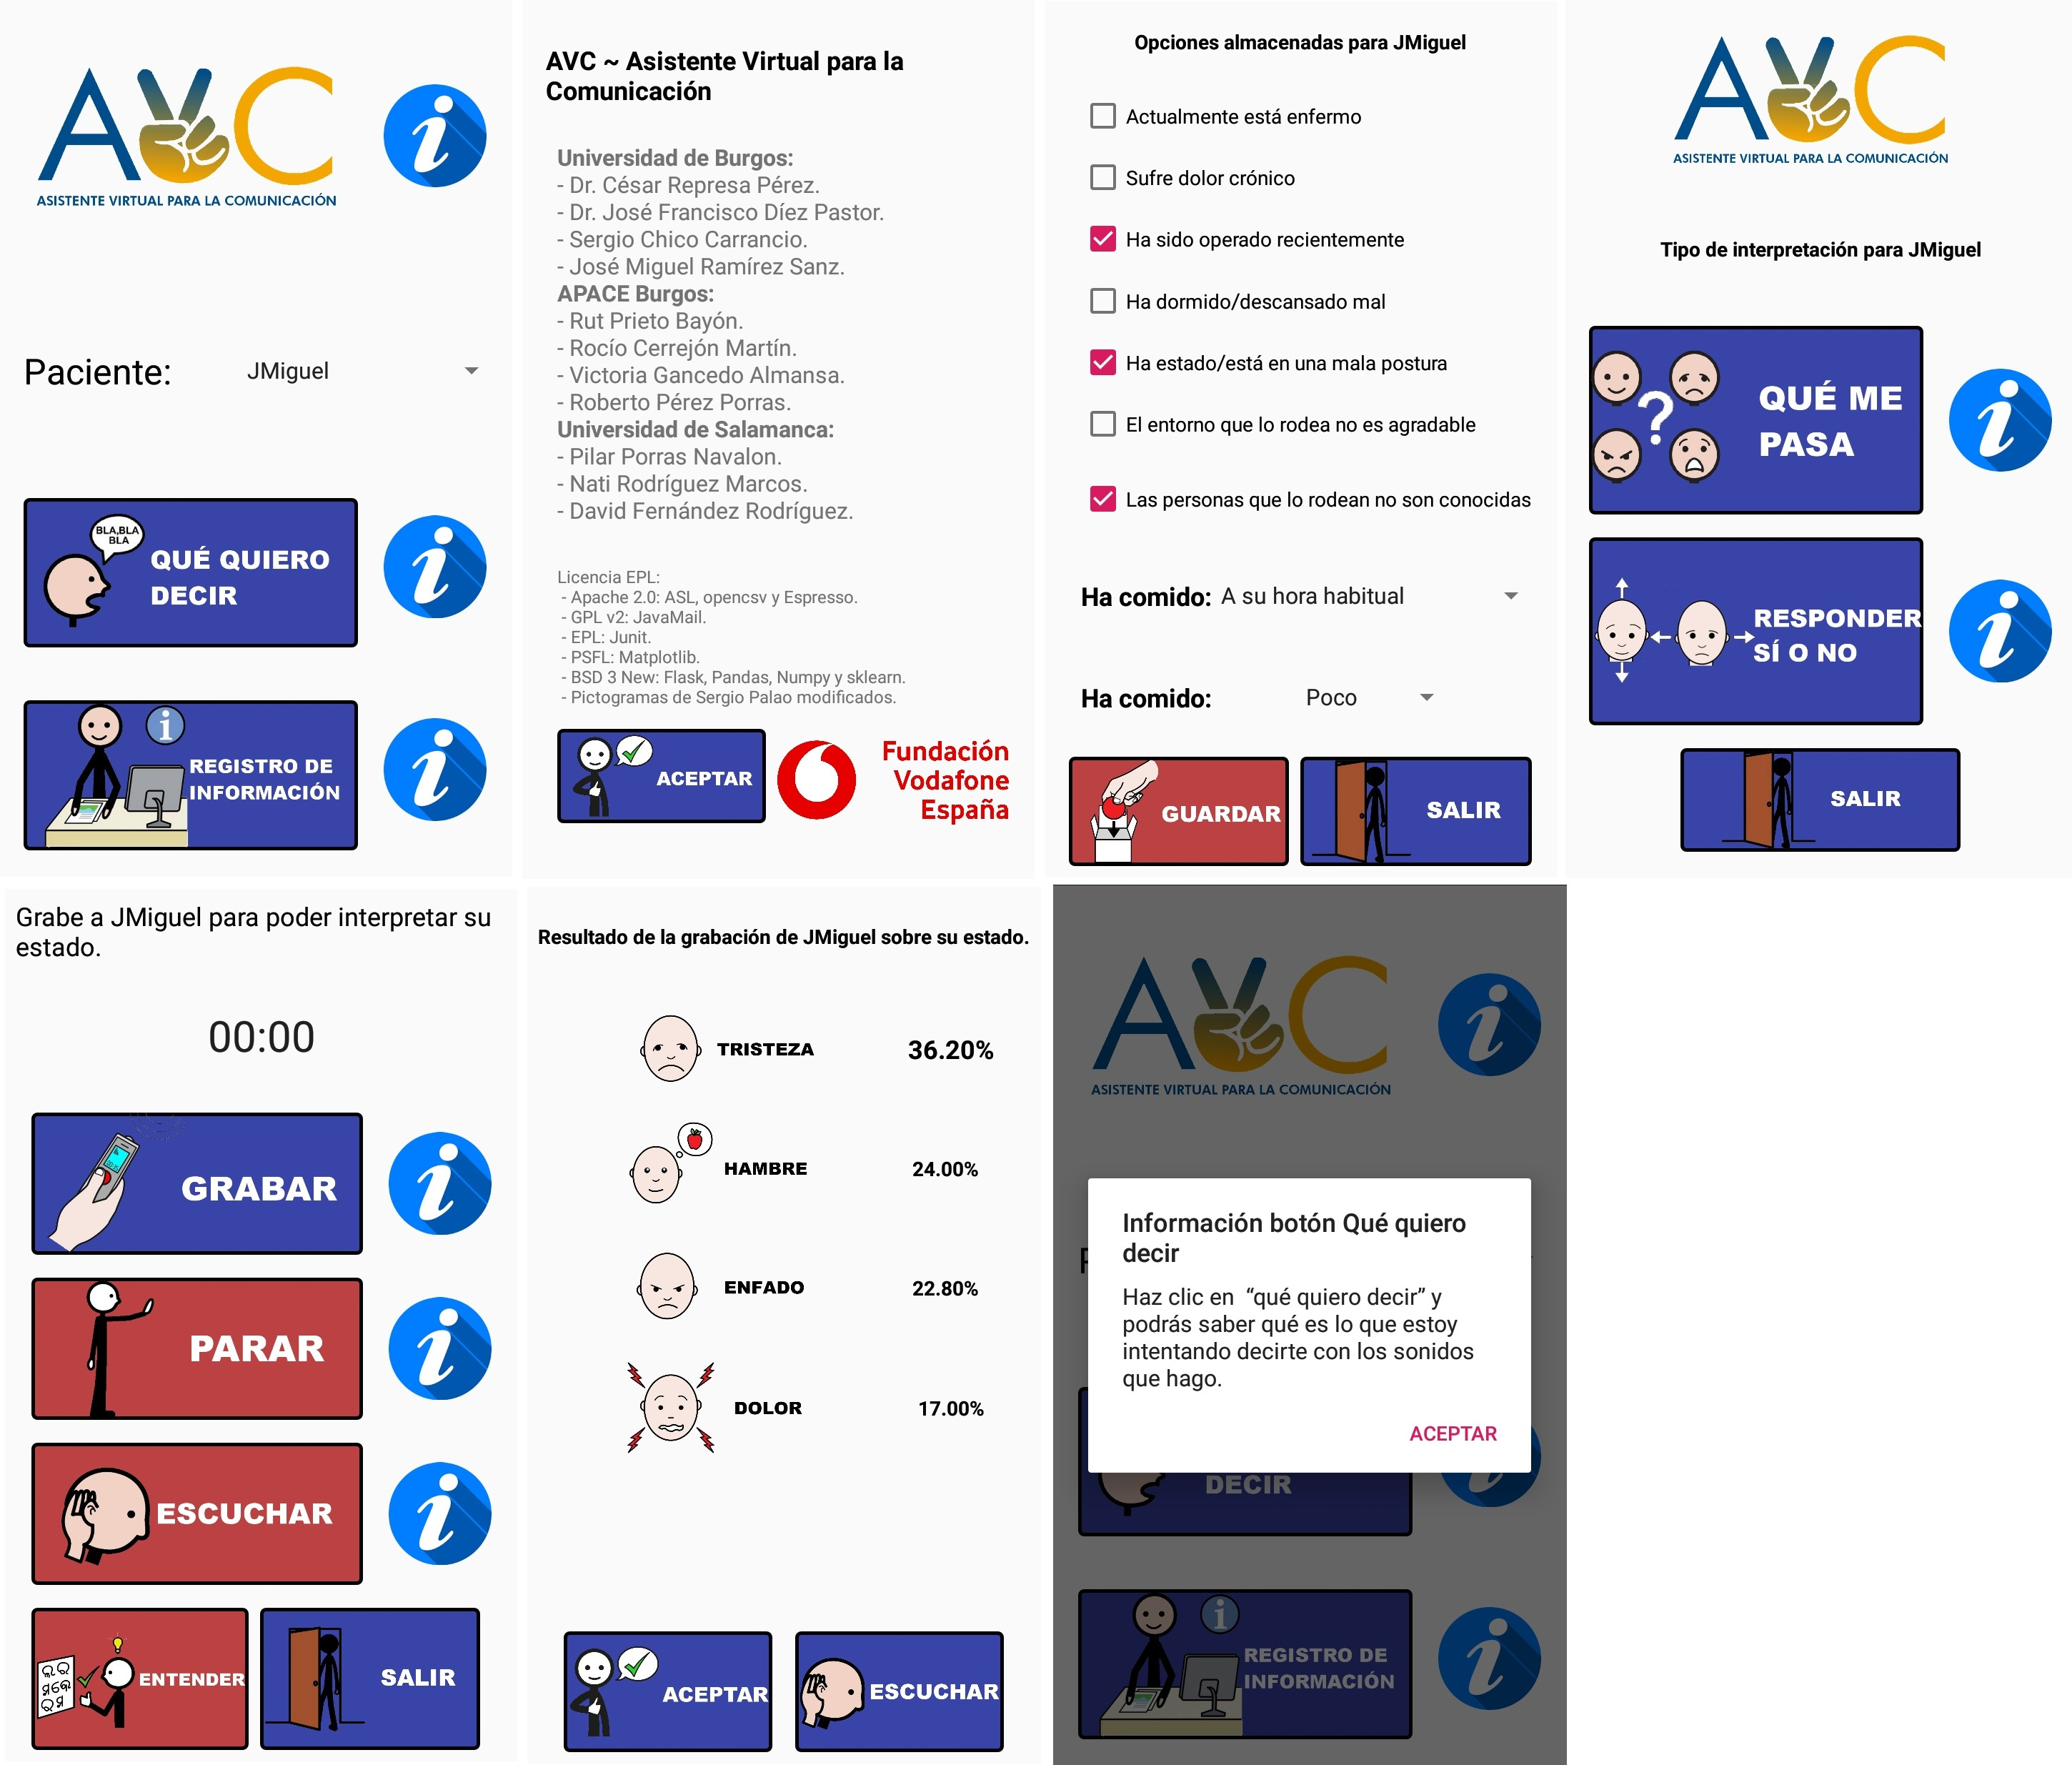
\includegraphics[width=\textwidth]{interavc}
	\caption{Interfaz final de la aplicación AVC.}
	\label{fig:intfin}
\end{figure}

\section{Diseño de código de errores}
Mientras estaba desarrollando el servidor, e implementando su conexión con la aplicación, me dí cuenta de que los errores de los diferentes métodos se repetían continuamente. Es por ello que decidí diseñar un estándar de códigos de errores para así poder responder mejor ante un posible fallo en la conexión entre la aplicación y el servidor, documentando la causa del fallo y como poder arreglarlo. El diseño del código de errores se puede ver en la figura~\ref{tabla:errores}.

\begin{table}[H]
	\resizebox{\textwidth}{!}{%
	\begin{tabular}{@{}llll@{}}
		\toprule
		Error & \textbf{Descripción}                                                                & \textbf{Causa}                                                                                                                                                                               & \textbf{Solución}                                                                                                                                    \\ \midrule
		Er1   & \begin{tabular}[c]{@{}l@{}}No se puede \\ acceder al servidor.\end{tabular}         & \begin{tabular}[c]{@{}l@{}}Este error se da cuando el servidor\\  está caído.\end{tabular}                                                                                                   & \begin{tabular}[c]{@{}l@{}}Avisar al Administrador para que \\ reinicie el servidor.\end{tabular}                                                    \\
		Er2   & \begin{tabular}[c]{@{}l@{}}Token de \\ seguridad\\  incorrecto.\end{tabular}        & \begin{tabular}[c]{@{}l@{}}O se ha corrompido la aplicación\\  cambiando el token de seguridad \\ o el token de seguridad ha cambiado\\  sin ser actualizado en su dispositivo.\end{tabular} & \begin{tabular}[c]{@{}l@{}}Avisar al Administrador para que \\ le pase de nuevo la aplicación.\end{tabular}                                          \\
		Er3   & \begin{tabular}[c]{@{}l@{}}Lista de nombres \\ vacía en el servidor.\end{tabular}   & \begin{tabular}[c]{@{}l@{}}La lista con los nombres en el\\  servidor está vacía.\end{tabular}                                                                                               & \begin{tabular}[c]{@{}l@{}}Avisar al Administrador para \\ que recupere el archivo.\end{tabular}                                                     \\
		Er4   & \begin{tabular}[c]{@{}l@{}}Lista de nombres \\ no encontrada.\end{tabular}          & \begin{tabular}[c]{@{}l@{}}El fichero con la lista de los \\ pacientes en el servidor no está.\end{tabular}                                                                                  & \begin{tabular}[c]{@{}l@{}}Avisar al Administrador para \\ que recupere el archivo.\end{tabular}                                                     \\
		Er5   & \begin{tabular}[c]{@{}l@{}}Opciones del \\ paciente no\\  encontradas.\end{tabular} & \begin{tabular}[c]{@{}l@{}}El fichero con las opciones \\ adicionales del paciente no \\ está en el servidor.\end{tabular}                                                                   & \begin{tabular}[c]{@{}l@{}}Avisar al Administrador para \\ que recupere el archivo.\end{tabular}                                                     \\
		Er6   & \begin{tabular}[c]{@{}l@{}}No hay \\ conexión \\ a Internet.\end{tabular}           & \begin{tabular}[c]{@{}l@{}}No tener conexión ni Wifi \\ ni Datos Móviles.\end{tabular}                                                                                                       & \begin{tabular}[c]{@{}l@{}}Conectarse a una red con acceso\\  a Internet.\end{tabular}                                                               \\
		Er7   & \begin{tabular}[c]{@{}l@{}}Fichero del \\ paciente vacío.\end{tabular}              & \begin{tabular}[c]{@{}l@{}}El fichero del paciente con las\\  opciones está vacío en el servidor.\end{tabular}                                                                               & \begin{tabular}[c]{@{}l@{}}Avisar al Administrador para \\ que recupere el archivo.\end{tabular}                                                     \\
		Er8   & \begin{tabular}[c]{@{}l@{}}Fichero de \\ clasificación \\ no existe.\end{tabular}   & \begin{tabular}[c]{@{}l@{}}No existe el fichero con el que se\\  clasifica en el servidor a ese paciente.\end{tabular}                                                                       & \begin{tabular}[c]{@{}l@{}}Avisar al Administrador para \\ que recupere el archivo.\end{tabular}                                                     \\
		Er9   & Resultado vacío.                                                                    & \begin{tabular}[c]{@{}l@{}}El servidor ha devuelto una \\ solución vacía.\end{tabular}                                                                                                       & \begin{tabular}[c]{@{}l@{}}Avisar al Administrador para \\ que compruebe el funcionamiento \\ de la clasificación para ese\\  paciente.\end{tabular} \\ \bottomrule
	\end{tabular}
	}
	\caption{Código de errores.}
	\label{tabla:errores}
\end{table}

